\begin{figure}[t]
\centering
\begin{subfigure}{0.37\columnwidth}
	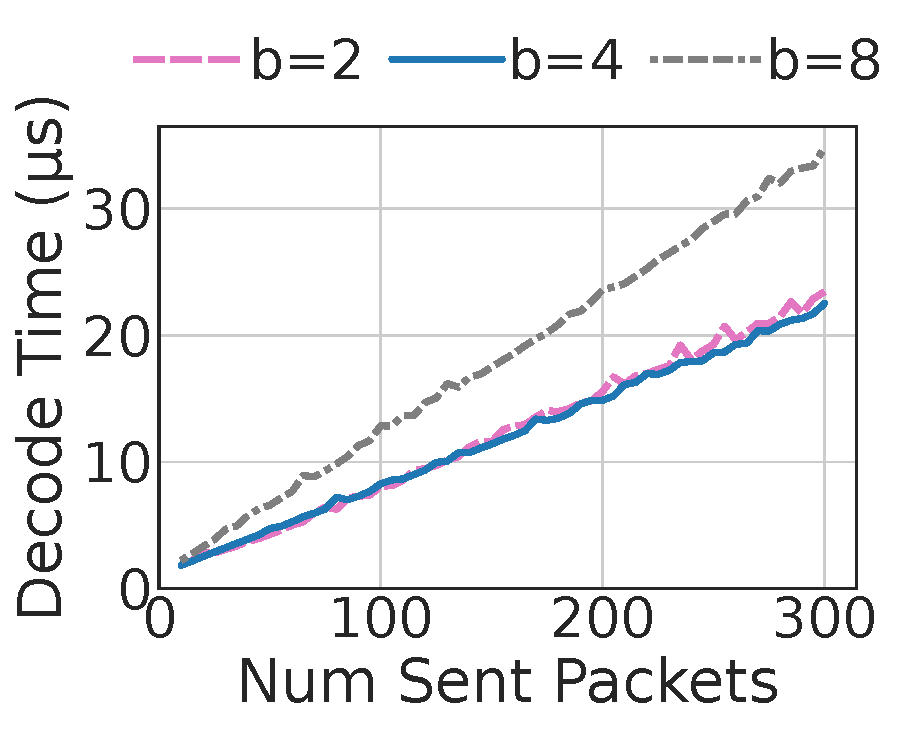
\includegraphics[width=\linewidth,trim={3mm 0 7mm 0},clip]{quack/figures/fig2a_quack_num_candidates_vs_decode_time.pdf}
	\caption{$n$ vs. decode time, where $t=m=10$.}
	\label{fig:quack:psum-decode:n}
\end{subfigure}
\begin{subfigure}{0.4\columnwidth}
	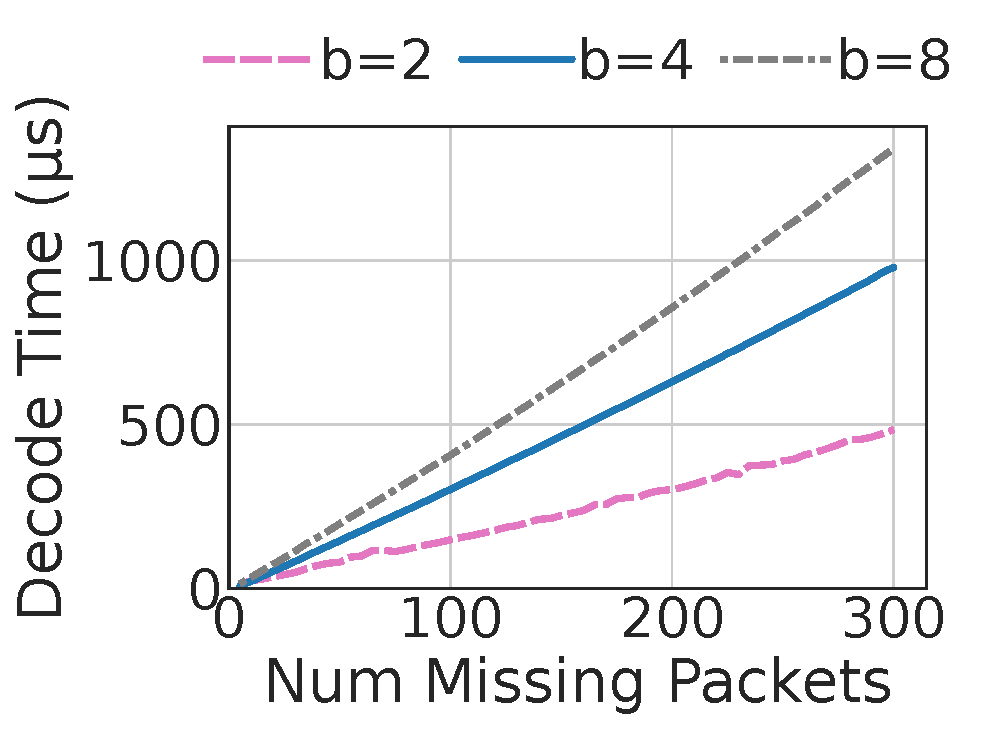
\includegraphics[width=\linewidth,trim={3mm 0 7mm 0},clip]{quack/figures/fig2b_quack_num_missing_vs_decode_time.pdf}
	\caption{$m$ vs. decode time, where $n=300$.}
	\label{fig:quack:psum-decode:m}
\end{subfigure}
\caption{The decoding time of the power sum quACK scales linearly with both the
 number of candidate (sent) packets $n$ and the number of missing packets $m$.
 Higher bit widths generally indicate higher computation costs. The typical
 decoding time is in microseconds. Average of 100 trials. }
\label{fig:quack:psum-decode}
\end{figure}
